\documentclass[a4paper]{report}
\usepackage[utf8]{inputenc}
\usepackage[portuguese]{babel}
\usepackage{hyperref}
\usepackage{a4wide}
\hypersetup{pdftitle={GestVendas},
pdfauthor={José Ferreira, João Teixeira},
colorlinks=true,
urlcolor=blue,
linkcolor=black}
\usepackage{subcaption}
\usepackage[cache=false]{minted}
\usepackage{listings}
\usepackage{booktabs}
\usepackage{multirow}
\usepackage{appendix}
\usepackage{tikz}
\usepackage{authblk}
\usetikzlibrary{positioning,automata,decorations.markings}

\begin{document}

\title{GestVendas\\ 
\large Grupo Nº 56}
\author{José Ferreira (A83683) \and João Teixeira (A85504)}
\date{\today}

\begin{center}
    \begin{minipage}{0.75\linewidth}
        \centering
        
\includegraphics[width=0.4\textwidth]{eng.jpeg}\par\vspace{1cm}
        \vspace{1.5cm}
        \href{https://www.uminho.pt/PT}
        {\color{black}{\scshape\LARGE Universidade do Minho}} \par
        \vspace{1cm}
        \href{https://www.di.uminho.pt/}
        {\color{black}{\scshape\Large Departamento de Informática}} \par
        \vspace{1.5cm}
        \maketitle
    \end{minipage}
\end{center}

\tableofcontents

\pagebreak

\chapter{Introdução}

O objetivo deste projeto é construir um sistema de gestão de vendas modular,
de forma a ser capaz de armazenar informações de vendas e relacionar produtos,
clientes e vendas de forma eficiente, aplicando uma arquitetura \textit{Model, View,
Controller} e conhecimentos sobre algoritmos e estruturas de dados. Como objetivo, 
é também necessário garantir o encapsulamento dos dados armazenados de forma
a que não sejam possíveis alterações indevidas por agentes externos.\\
Ao longo deste relatório vamos descrever as nossas abordagens a estes problemas e
apresentar alguns testes de performance do nosso projeto final.

\chapter{Problema}
Três ficheiros são fornecidos contendo informação sobre as transações de uma distribuidora:
\begin{itemize}
    \item O primeiro contém ids de produtos.
    \item Outro, ids de clientes.
    \item O último integra informações sobre cada venda efetuada ao longo de um ano. 
\end{itemize}
Com base nesses ficheiros é preciso responder a 12 queries fornecidas:
\begin{enumerate}
    \item Estatísticas sobre os ficheiros lidos.
    \item Números gerais sobre os dados carregados.
    \item Lista dos códigos de produtos não comprados.
    \item Número de vendas realizadas e clientes distintos, num dado mês e numa dada filial.
    \item Número de produtos distintos e gastos totais mês a mês para um dado cliente.
    \item Determinar mês a mês quantas vezes foi comprado, por quantos clientes e o total facturado de um dado produto.
    \item Produtos mais comprados por um dado cliente e a sua quantidade.
    \item X produtos mais vendidos todo o ano e o número de clientes que o compraram.
    \item Determinar os 3 maiores compradores em cada filial.
    \item X clientes que compraram mais produtos diferentes e quantos.
    \item X clientes que compraram um dado produto e qual o valor gasto.
    \item Calculara a facturação total de um dado produto, mês a mês e filial a filial.
\end{enumerate}

\chapter{Módulos e API}\label{chap:api}

Tendo em conta as características do projeto, concluímos que a arquitetura que melhor
abrangia os critérios pedidos era a Arquitetura do tipo \textit{MVC} (Modelo, 
Apresentação e Controlador).
Um dos critérios que mais fez o grupo gravitar em direcção a esta escolha foi 
a modularidade inerente a esta arquitetura.

\section{Model}

\subsection{Cliente}

O módulo de Cliente tem uma API capaz de lidar com a informação de um cliente
individual, e sua respetiva validação. 

\subsection{Clientes}

O módulo de Clientes tem uma API capaz de lidar com a informação de todos os
clientes, respectivo armazenamento e pesquisa. \\ 
Como estrutura principal de armazenamento dos Clientes individuais, após testes 
testar várias estruturas, optamos por utilizar os HashMaps presente na biblioteca
\textit{java.util.Map}

\subsection{Produto}

À semelhança do módulo de Cliente, o módulo de Produto tem uma API desenhada
para tratar da informação referente a um produto individual, bem como a sua 
validação

\subsection{Produtos}

No módulo de Produtos, a API está construída de maneira a que seja capaz de
lidar, de forma eficiente com o armazenamento e pesquisa de todos os produtos.\\
Para este módulo, como no módulo de Clientes, decidimos utilizar os mesmos HashMaps
da biblioteca \textit{java.util.Map}

\subsection{Venda}

No módulo de Venda, temos uma API capaz de dar parse de uma string com o formato 
previamente definido, colocar numa estrutura com os campos necessários de maneira
a preservar a informação, para posteriormente ser tratada pelo módulo de Filiais e
Facturação.

\subsection{Factura}

Neste módulo, a API está definida de forma a conseguir, a partir de uma Venda,
criar/actualizar uma factura, contendo esta, a facturação relativa a um produto.

\subsection{Faturas}

O módulo de Faturas é capaz de comportar informação sobre toda a faturação,
organizada por produtos e guardada numa Hashtable. Uma estrutura do tipo Faturas
para além de guardar a faturação individual de cada produto, para um mais rápido 
acesso, guarda também valores totais de faturação e número de vendas.

\subsection{Filial}

Para o módulo de filial, está definida uma API capaz de fazer a ligação entre 
clientes e os respetivos produtos por eles comprados, e vice-versa.\\
Uma estrutura do tipo Filial é composta por duas Hashtables, uma que contém
informação relativa a todos os clientes que fizeram compras na dada filial, 
que produtos compraram e respetiva faturação, e uma segunda que contém 
informação relativa a todos os produtos vendidos na dada filial, mais 
concretamente que clientes adquiriram o produto.

\subsection{Constantes}

No módulo constantes, são guardadas todas as informações referentes ao número de
filiais, ficheiros a ler, entre outros, que são lidas de um ficheiro de configs

\subsection{GestVendasModel}

O módulo GestVendasModel é o módulo que junta todos os acima descritos, 
contendo este uma estrutura
que contém um Catálogo de Produtos, um Catálogo de Clientes, uma estrutura Faturação e 
um array de Filiais. Este módulo faz a ponte entre todos os módulos internos e o 
exterior, sendo este o módulo que ao qual o controlador faz pedidos, e tem 
métodos capazes de responder a todas as queries pedidas.

\section{View}

Esta \textit{package} contém as classes de apresentação dos resultados ao utilizador.

\subsection{GestVendasView}

Esta classe representa os vários Menus e as relações entre eles. Para permitir
conhecer o caminho percorrido até ao menu que se está a observar esta classe
contém uma stack com os menus percorridos.

\subsection{Navigator}

A fim de facilitar a apresentação de determinadas queries foi criada uma classe que 
apresenta uma lista de valores sobre a forma de páginas.\\
De forma a que esta representação se ajuste ao terminal que está a ser utilizado, 
o número de linhas e de colunas que vai ser representado em cada página navegável 
é calculado com base no tamanho do terminal presente. Para tal, a classe Terminal 
é utilizada.

\subsection{Table}

Alguns dos dados obtidos nas queries variam em duas variáveis discretas finitas, como por exemplo
ao mês a mês e filial a filial em simultâneo.\\
Assim, naturalmente, a melhor forma de representar tais dados é através de uma tabela.
Para tal foi desenvolvida uma classe para representar tabelas com um 
\textit{generic type parameter}.\\
Consequentemente, esta classe apenas precisa de duas listas de etiquetas (uma 
para as linhas e outra para as colunas) e uma Lista de Listas com os dados para 
representar uma tabela visualmente apelativa em que cada coluna automaticamente 
adapta o seu tamanho ao seu conteúdo.

\section{Controller}

Cria a ponte entre o View e o Model. Assim, o Controller é o único que conhece a view e o
Model, sendo que tanto a View como o Model apenas conhecem o Controller.

\subsection{GestVendasController}

Esta classe actua como o controlador do nosso projeto. Para além de funcionar como a ponte entre
a lógica e a apresentação também cronometra o tempo demorado pela lógica a responder às queries pedidas
e passa esse valor à \textit{View} para ser apresentado ao utilizador.

\section{Exceptions}

Esta Package contém todas as classes de exceções utilizadas ao longo do projeto.
Estas são usadas para assinalar, por exemplo, uma filial ou um cliente inválido passado
como argumento.

\section{Utils}

A \textit{package} Utils contém classes que são utilizadas em várias partes do projeto e que não
pertencem a uma parte específica da arquitetura \textit{MVC}.

\subsection{Crono}

A Classe Crono está desenhada para medir o tempo decorrido ao longo da execução do projeto.
Para tal possui dois métodos, o \textit{start} e o \textit{stop} que devem ser chamados no
inicio e no fim da porção de código que se quer cronometrar, respetivamente.
Por fim, para apresentar o resultado ao utilizador, a função \textit{toString} foi implementada
de forma a apresentar os tempos calculados de forma legível.

\subsection{Terminal}

A classe Terminal calcula o tamanho do terminal onde o programa está a correr.
Para tal realiza duas \textit{System Calls} com dois \textit{Fork exec} (uma para obter a altura
e outra para obter a largura do terminal).
Para recalcular o tamanho basta chamar o método \textit{update}.

\subsection{StringBetter}

A Classe StringBetter contém métodos que permitem formatar texto quando este é impresso na
\textit{Shell}. Estes métodos incluem mudar a cor, negrito e itálico e repetir o texto N vezes.\\
Afim de agilizar a utilização da classe, todos os métodos devolvem uma instância da classe
de forma a ser possível o encadeamento de métodos.\\
Assim, se um utilizador quiser escrever \textit{Hello World} a negrito, sublinhado e a
vermelho basta escrever.
\begin{figure}[H]
    \begin{center}
        \begin{verbatim}
        out.println(new StringBetter("Hello World").bold().under().red()
        \end{verbatim}
    \end{center}
\end{figure}

\chapter{Arquitetura do projeto}

\section{Modelo}

O modelo tem como base dois grandes módulos, o módulo Filial e o módulo Facturação,
e têm como módulos auxiliares ambos os Catálogos de Produtos e de Clientes.\\
Estes dois grandes módulos estão unidos num módulo mais geral, GereVendasModel, 
e este recebe os pedidos do GereVendasController, e trata a informação contida 
em todos os módulos, de forma a devolver-lhe a informação pedida da forma mais 
eficiente. É nesta camada onde está toda a parte de algoritmos e dados, nunca 
esta conhecendo ou dada a conhecer à camada da Apresentação.

\chapter{Testes e Benchmarks}

Durante a execução do nosso projeto, foram efetuados diversos testes, quer ao nível
de formas de leitura do ficheiro, em particular, \textit{BufferedReader} e \textit{Files},
bem como testes ao nível das diversas implementações das Interfaces \textit{Map},
\textit{Set} e \textit{List}

\section{Tempos de execução}

Com recurso à classe fornecida \textit{Crono}, efetuamos alguns benchmarks, obtendo
a tabela \ref{tab:benches}, com os tempos médios de execução, com os diversos ficheiros
de vendas fornecidos.\\
Nestes vários benchmarks, testamos diferentes implementações das Interfaces \textit{Map},
nomeadamente, \textit{HashMap} e \textit{TreeMap}, concluindo assim que os tempos de 
que os \textit{HashMap} são muito mais rápidos no carregamento da informação para 
memória, mantendo os tempos das queries praticamente inalterados, como é possível
comprovar na tabela \ref{tab:benchesTH}.\\
Foram também testados tempos de execução das Implementações da Interface \textit{List},
nomeadamente \textit{ArrayList} e \textit{Vector}, visivel na tabela \ref{tab:benchesLV}
não havendo diferenças notáveis, acabando assim por optar pela implementação 
mais comum \textit{ArrayList}.\\
Ao nível de leitura, foram efetuados benchmarks para comparar a performance de
\textit{Files} e de \textit{BufferedReader} vistos em no apêndice \ref{chap:brf}, sendo o
\textit{Files} mais lento e já que internamente \textit{Files} utiliza internamente
\textit{BufferedReader}, acabamos por utilizar o \textit{BufferedReader} para a leitura
dos ficheiros com a informação.

\chapter{Conclusão}

Para concluir, conseguimos cumprir todos os requisitos propostos, conseguindo implementar
todos os módulos e estrutura-los como pedido, sendo assim capaz de responder a todas as 
queries da forma que nos pareceu mais eficiente.\\
Como trabalho futuro, gostariamos de melhorar a maneira da organização da informação 
referente às filiais, de forma a baixar tempo de resposta a queries que utilizam informação
nele presente.

\appendix

\chapter{Diagramas de Classes}
\begin{figure}[H]
    \begin{center}
        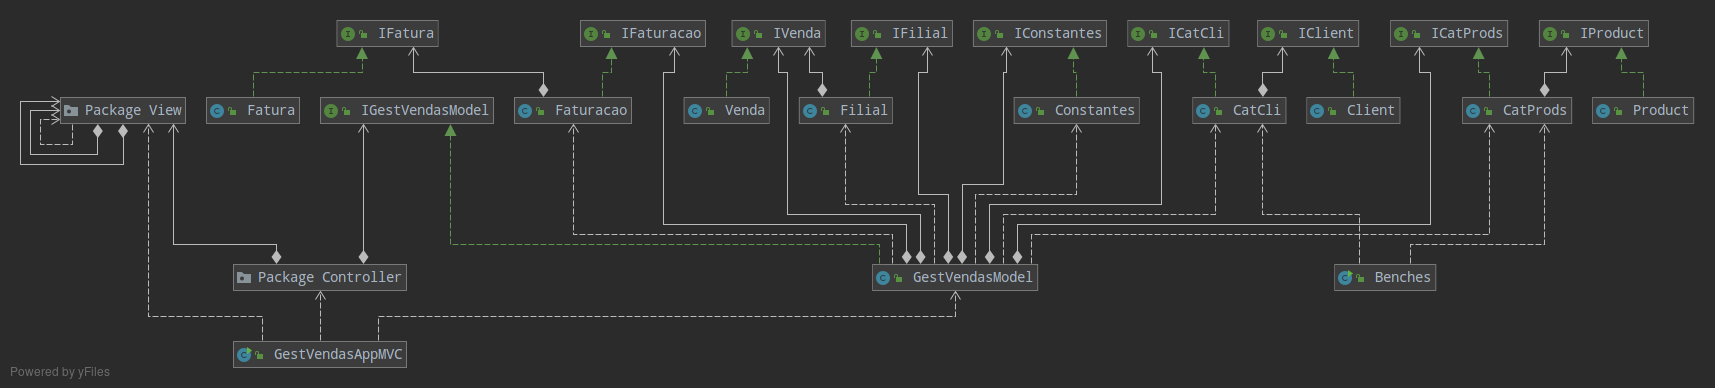
\includegraphics[width=1\textwidth]{modelGraph.png}\par
        \caption{Diagrama de Classes do Model}
    \end{center}
\end{figure}

\begin{figure}[H]
    \begin{center}
        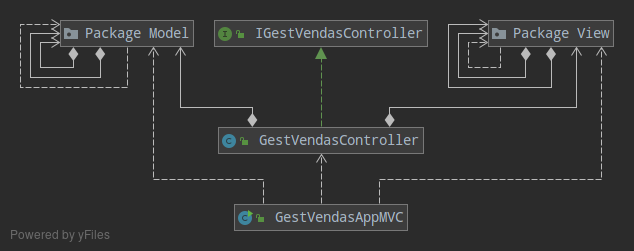
\includegraphics[width=1\textwidth]{viewGraph.png}\par
        \caption{Diagrama de Classes do Controller}
    \end{center}
\end{figure}

\begin{figure}[H]
    \begin{center}
        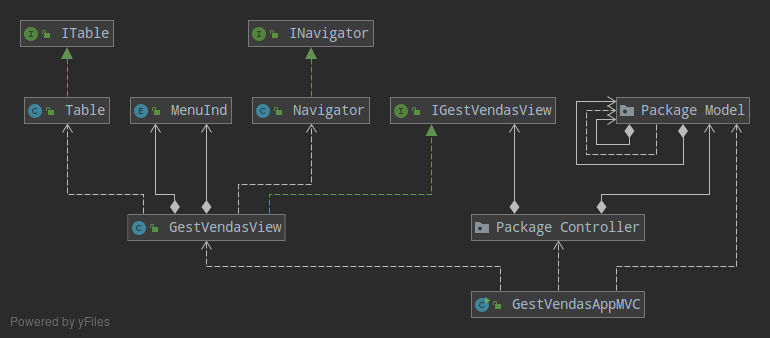
\includegraphics[width=1\textwidth]{controllerGraph.png}\par
        \caption{Diagrama de Classes do View}
    \end{center}
\end{figure}

\chapter{Benchmarks BufferedReader vs Files}\label{chap:brf}

\begin{table}[H]
    \begin{center}
        \begin{tabular}{| c | c | c | c |}
            \hline
            & 1 Milhão & 3 Milhões & 5 Milhões \\
            \hline
            Leitura & 162 & 434 & 750 \\
            \hline
            Parse & 871 & 1884 & 3013 \\
            \hline
            Validação & 1316 & 3120 & 4380 \\
            \hline
            Validação Paralela & 795 & 1535 & 2203 \\
            \hline

        \end{tabular}
        \caption{Tempo (em ms) de tempos de BufferedReader} 
        \label{tab:BF}
    \end{center}
\end{table}

\begin{table}[H]
    \begin{center}
        \begin{tabular}{| c | c | c | c |}
            \hline
            & 1 Milhão & 3 Milhões & 5 Milhões \\
            \hline
            Leitura & 173 & 480 & 773 \\
            \hline
            Parse & 861 & 1948 & 3017 \\
            \hline
            Validação & 1139 & 2755 & 4380 \\
            \hline
            Validação Paralela & 828 & 1572 & 2222 \\
            \hline

        \end{tabular}
        \caption{Tempo (em ms) de tempos Files}
        \label{tab:Files}
    \end{center}
\end{table}


\chapter{Tabela de Tempos de Execução}

\begin{table}[H]
    \begin{center}
        \begin{tabular}{| c | c | c | c |}
            \hline
            & 1 Milhão & 3 Milhões & 5 Milhões \\
            \hline
            Load Time & 2002 & 4522 & 7359 \\
            \hline
            Query 1 & 68 & 32 & 31 \\
            \hline
            Query 2 & 39 & 80 & 119 \\
            \hline
            Query 3 & 55 & 20 & 14 \\
            \hline
            Query 4 & 1 & 1 & 1 \\
            \hline
            Query 5 & 13 & 22 & 17 \\
            \hline
            Query 6 & 950 & 2306 & 3730 \\
            \hline
            Query 7 & 71 & 111 & 72 \\
            \hline
            Query 8 & 240 & 1115 & 1526 \\
            \hline
            Query 9 & 9 & 14 & 10 \\
            \hline
            Query 10 & 45 & 100 & 230 \\
            \hline

        \end{tabular}
        \caption{Tempo (em ms) das queries para um dado número de vendas}
        \label{tab:benches}
    \end{center}
\end{table}

\begin{table}[H]
    \begin{center}
        \begin{tabular}{| c | c | c | c |}
            \hline
            & 1 Milhão & 3 Milhões & 5 Milhões \\
            \hline
            Load Time & 2117 & 4824 & 7270 \\
            \hline
            Query 1 & 21 & 32 & 34 \\
            \hline
            Query 2 & 78 & 86 & 117 \\
            \hline
            Query 3 & 5 & 20 & 18 \\
            \hline
            Query 4 & 1 & 1 & 1 \\
            \hline
            Query 5 & 11 & 26 & 18 \\
            \hline
            Query 6 & 858 & 2405 & 3942 \\
            \hline
            Query 7 & 67 & 121 & 57 \\
            \hline
            Query 8 & 267 & 900 & 1418 \\
            \hline
            Query 9 & 7 & 5 & 10 \\
            \hline
            Query 10 & 33 & 104 & 176 \\
            \hline

        \end{tabular}
        \caption{Tempo (em ms) das queries para um dado número de vendas, utilizando
        \textit{Vector} em vez de \textit{ArrayList}}
        \label{tab:benchesLV}
    \end{center}
\end{table}

\begin{table}[H]
    \begin{center}
        \begin{tabular}{| c | c | c | c |}
            \hline
            & 1 Milhão & 3 Milhões & 5 Milhões \\
            \hline
            Load Time & 5060 & 16100 & 25369 \\
            \hline
            Query 1 & 74 & 32 & 27 \\
            \hline
            Query 2 & 69 & 88 & 94 \\
            \hline
            Query 3 & 45 & 10 & 18 \\
            \hline
            Query 4 & 1 & 2 & 1 \\
            \hline
            Query 5 & 48 & 15 & 14 \\
            \hline
            Query 6 & 929 & 2528 & 3690 \\
            \hline
            Query 7 & 62 & 68 & 80 \\
            \hline
            Query 8 & 269 & 816 & 1430 \\
            \hline
            Query 9 & 7 & 5 & 10 \\
            \hline
            Query 10 & 50 & 111 & 155 \\
            \hline

        \end{tabular}
        \caption{Tempo (em ms) das queries para um dado número de vendas, utilizando
        \textit{TreeMap} em vez de \textit{HashMap}}
        \label{tab:benchesTH}
    \end{center}
\end{table}


\end{document}
